\documentclass[tikz,border=4pt]{standalone}
\usepackage[T1]{fontenc}
\usepackage[utf8]{inputenc}
\usepackage{amsmath,amssymb}
\usepackage{helvet}
\renewcommand{\familydefault}{\sfdefault}
\usepackage{pgfplots}
\pgfplotsset{compat=1.17}
\usetikzlibrary{arrows.meta,positioning,calc,fit,backgrounds,shapes.geometric}

\definecolor{cVis}{HTML}{1F77B4}
\definecolor{cTxt}{HTML}{D62728}
\definecolor{cProj}{HTML}{2CA02C}
\definecolor{cLLM}{HTML}{9467BD}
\definecolor{cConv}{HTML}{FF7F0E}
\definecolor{cAtt}{HTML}{17BECF}
\definecolor{cGray}{HTML}{7F7F7F}

\tikzset{
  blk/.style={draw, rounded corners=2pt, minimum height=8mm, align=center, font=\footnotesize, thick},
  tok/.style={draw, minimum size=3.2mm, inner sep=0pt},
  arr/.style={-{Stealth[length=2mm]}, thick},
}

\begin{document}
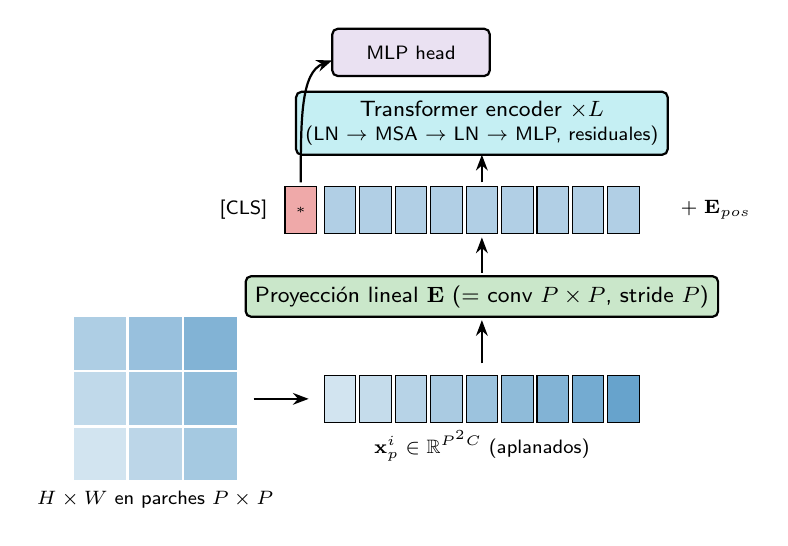
\begin{tikzpicture}[x=1cm,y=1cm]
  \foreach \i in {0,1,2}{\foreach \j in {0,1,2}{
    \pgfmathsetmacro{\c}{20+10*\i+8*\j}
    \fill[cVis!\c] (\i*0.7,\j*0.7) rectangle ++(0.7,0.7);
    \draw[white,thick] (\i*0.7,\j*0.7) rectangle ++(0.7,0.7);}}
  \node[below, font=\scriptsize] at (1.05,0) {$H\times W$ en parches $P\times P$};
  \draw[arr] (2.3,1.05) -- (3.0,1.05);
  \foreach \k in {0,...,8}{\pgfmathsetmacro{\c}{20+6*\k}\node[tok,fill=cVis!\c,minimum width=4mm,minimum height=6mm] at (3.4+\k*0.45,1.05) {};}
  \node[font=\scriptsize] at (5.2,0.45) {$\mathbf{x}_p^i\in\mathbb{R}^{P^2C}$ (aplanados)};
  \draw[arr] (5.2,1.5) -- (5.2,2.05);
  \node[blk, fill=cProj!25, minimum width=46mm, minimum height=5mm] at (5.2,2.35) {Proyección lineal $\mathbf{E}$ (= conv $P\times P$, stride $P$)};
  \draw[arr] (5.2,2.65) -- (5.2,3.1);
  \node[tok,fill=cTxt!40,minimum width=4mm,minimum height=6mm] at (2.9,3.45) {\tiny$\ast$};
  \foreach \k in {0,...,8}{\node[tok,fill=cVis!35,minimum width=4mm,minimum height=6mm] at (3.4+\k*0.45,3.45) {};}
  \node[font=\scriptsize, anchor=west] at (7.6,3.45) {$+\;\mathbf{E}_{pos}$};
  \node[font=\scriptsize, anchor=east] at (2.6,3.45) {[CLS]};
  \draw[arr] (5.2,3.8) -- (5.2,4.15);
  \node[blk, fill=cAtt!25, minimum width=46mm] at (5.2,4.55) {Transformer encoder $\times L$\\[-1pt]\scriptsize (LN $\to$ MSA $\to$ LN $\to$ MLP, residuales)};
  \draw[arr] (2.9,3.8) .. controls (2.9,4.6) and (2.9,5.2) .. (3.3,5.35);
  \node[blk, fill=cLLM!20, minimum width=20mm, minimum height=6mm] at (4.3,5.45) {\scriptsize MLP head};
\end{tikzpicture}
\end{document}
